\documentclass[final]{article}

\usepackage{APS360}
\usepackage[utf8]{inputenc}
\usepackage[T1]{fontenc}
\usepackage{hyperref}
\usepackage{url}
\usepackage{booktabs}
\usepackage{amsmath}
\usepackage{microtype}
\usepackage{xcolor}
\usepackage{graphicx}
\usepackage{tabularx}
\usepackage{tikz}
\usetikzlibrary{arrows.meta,positioning}

\definecolor{motionblue}{HTML}{D9EAF7}
\definecolor{modelgreen}{HTML}{DCEED1}
\definecolor{outputorange}{HTML}{FCE2C4}

\title{Early Prediction of Human Engagement Intent for Social Robot Interaction}

\author{%
  Asser Abdelgawad \\
  1008107567, \texttt{asser.abdelgawad@mail.utoronto.ca} \\
  \href{https://github.com/asso-the-coder/robot-predicting-interactions-with-humans}{Code and experiment repository}%
}

\begin{document}

\maketitle
\vspace{-0.45in}

\section*{Introduction}

A public-facing robot must decide whether a nearby person is approaching to interact or simply passing through its field of view. Acting too early can interrupt a passerby, while acting too late can make the robot appear unresponsive. This project treats early engagement prediction as supervised binary classification. Given a short robot-centric sequence observed before engagement begins, the system predicts whether that person will interact within four seconds. Machine learning is appropriate because intent is not identified by one measurement. It is expressed through a temporal combination of distance, speed, direction, body orientation, and pose. The practical scope is deliberately low risk: the prediction could support greeting, waiting, or avoiding an interruption, but not surveillance or consequential decisions.

\section*{Illustration}

\begin{figure}[!h]
  \centering
  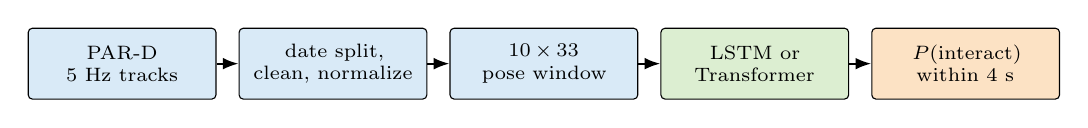
\begin{tikzpicture}[
    node distance=2.8mm,
    box/.style={draw, rounded corners=1.5pt, align=center, minimum height=9mm,
      text width=2.15cm, font=\scriptsize},
    arrow/.style={-{Latex[length=2mm]}, thick}
  ]
    \node[box, fill=motionblue] (raw) {PAR-D\\5 Hz tracks};
    \node[box, fill=motionblue, right=of raw] (prep) {date split, clean, normalize};
    \node[box, fill=motionblue, right=of prep] (window) {$10\!\times\!33$\\pose window};
    \node[box, fill=modelgreen, right=of window] (model) {LSTM or\\Transformer};
    \node[box, fill=outputorange, right=of model] (out) {$P(\mathrm{interact})$\\within 4 s};
    \draw[arrow] (raw) -- (prep);
    \draw[arrow] (prep) -- (window);
    \draw[arrow] (window) -- (model);
    \draw[arrow] (model) -- (out);
  \end{tikzpicture}
  \caption{The model observes a fixed pre-engagement sequence. Recording dates are separated before overlapping windows are formed, preventing adjacent observations from crossing splits.}
  \label{fig:pipeline}
\end{figure}

\section*{Background and Related Work}

PAR-D defines the closest prior task and contributes public-robot interaction trajectories, behavioral labels, and computational and human baselines \citep{thompson2024pard}. JRDB provides robot-centric multimodal perception in populated indoor and outdoor environments \citep{martinmartin2019jrdb}; JRDB-Social extends it with individual, group, and social-context annotations \citep{jahangard2024jrdbsocial}. These datasets show the value and difficulty of perception from a moving or public robot, but PAR-D is the only one used for training here. Social LSTM established recurrent modeling of pedestrian trajectories and interactions \citep{alahi2016social}. The original LSTM addresses long temporal dependencies through gated recurrent state \citep{hochreiter1997lstm}. Transformers replace recurrence with self-attention and require an explicit representation of temporal position \citep{vaswani2017attention}. This project compares both sequence families with a simpler logistic model, focusing on early interaction intent rather than trajectory generation.

\section*{Data Processing}

The CC0 PAR-D Shutter release contains 1,059 scenario CSV files from two university lobbies, sampled at 5 Hz \citep{thompson2024pard}. Auditing found 139,092 rows, 337 columns, and 2,429 unique $(\mathrm{lobby},\mathrm{scenario},\mathrm{person})$ tracks over 13 recording dates. A target is positive when the released time-to-engagement field is in $[0,4]$ seconds at the final observation. Any window containing current engagement is rejected. Label-construction fields, button events, robot actions, speech, and future-state columns are excluded.

Dates are assigned before windows are constructed: nine dates for training, August 11 and 18 for validation, and August 8 and 23 for final test. This prevents overlapping frames from the same collection day entering multiple splits. Two-second windows contain 10 contiguous frames; gaps above 0.31 seconds are rejected. Missing velocity at the first track sample is imputed, and every numeric feature is standardized using training data statistics only. The resulting 50,157 windows are strongly imbalanced (5.0\% positive).

\begin{table}[!h]
  \centering
  \small
  \caption{Processed two-second windows.}
  \label{tab:data}
  \begin{tabular}{lrrr}
    \toprule
    Split & Windows & Positive & Negative \\
    \midrule
    Train & 36,952 & 1,693 & 35,259 \\
    Validation & 7,618 & 344 & 7,274 \\
    Test & 5,587 & 479 & 5,108 \\
    \bottomrule
  \end{tabular}
\end{table}

Three nested feature sets support an ablation: motion (6 features), orientation (12), and centered pose (33). Pose adds pelvis-centered head, shoulder, wrist, and ankle coordinates. Centering removes lobby-specific global offsets. Table~\ref{tab:example} shows three frames from an actual de-identified positive pose window; the model receives all 10 frames and 33 features. The true output is $y=1$, meaning engagement begins within four seconds.

\begin{table}[!h]
  \centering
  \scriptsize
  \caption{Subset of one actual input sequence, before standardization.}
  \label{tab:example}
  \begin{tabular}{rrrrrr}
    \toprule
    Frame & Distance (m) & Speed (m/s) & Bearing cos & Bearing sin & Head-to-cart cos \\
    \midrule
    1 & 0.869 & 1.040 & 1.000 & 0.018 & -0.985 \\
    5 & 0.554 & 0.430 & 0.993 & 0.114 & -0.999 \\
    10 & 0.583 & 0.010 & 0.998 & 0.067 & -0.996 \\
    \bottomrule
  \end{tabular}
\end{table}

\section*{Architecture and Baseline}

The primary model is a two-layer LSTM with 64 hidden units per layer and dropout 0.2. The last-layer hidden state passes through dropout and a linear head to produce one raw logit. It has 58,689 trainable parameters for pose input. The comparison Transformer projects each 33-dimensional frame to 64 dimensions, prepends a learned classification token, and adds sinusoidal positions. Two pre-normalized encoder layers each use four attention heads, a 128-dimensional GELU feed-forward block, and dropout 0.25. A normalized classification-token embedding produces the logit. It has 69,505 parameters.

Both networks use AdamW, batches of 512, gradient clipping at 1.0, and weighted binary cross entropy with a training-only positive weight of 20.83. The LSTM uses learning rate $10^{-3}$ and weight decay $10^{-4}$; the Transformer uses $5\times10^{-4}$ and $10^{-3}$. Checkpoints, early stopping, and probability thresholds are selected by validation F1. Sigmoid is applied only for metrics.

The learned baseline is class-balanced logistic regression ($C=1$). For every temporal input feature it receives the mean, standard deviation, first value, and last value. The selected orientation model therefore has 48 inputs plus an intercept. A majority-class predictor is also reported as a sanity check.

\section*{Quantitative Results}

At seed 360, the pose LSTM gave the best validation F1, 0.345, compared with 0.284 for orientation logistic regression. Motion, orientation, and pose LSTM F1 scores were 0.289, 0.289, and 0.345. Pose-window F1 was 0.274, 0.345, and 0.284 for one, two, and three seconds, so two seconds was selected. Longer context also reduced the number of eligible windows.

Repeated seeds changed the conclusion. Across seeds 360, 361, and 362, LSTM validation F1 was $0.273\pm0.063$ and Transformer F1 was $0.274\pm0.016$ (sample standard deviation). The Transformer was more stable, but neither neural model exceeded the deterministic logistic result of 0.284 on average. A smaller, more regularized Transformer reached only 0.259 F1.

The model, features, two-second window, checkpoint, and threshold were frozen before reading the test dates. Table~\ref{tab:test} shows that the LSTM validation advantage did not transfer. Accuracy is included but is not the main measure: always predicting negative obtains 91.4\% test accuracy and zero positive-class F1.

\begin{table}[!h]
  \centering
  \small
  \caption{Final unseen-date test results. Thresholds were selected on validation F1.}
  \label{tab:test}
  \begin{tabular}{lrrrrr}
    \toprule
    Model & Threshold & Accuracy & Precision & Recall & F1 \\
    \midrule
    Orientation logistic & 0.80 & 0.861 & 0.239 & 0.284 & \textbf{0.260} \\
    Pose LSTM & 0.83 & 0.862 & 0.115 & 0.092 & 0.102 \\
    \bottomrule
  \end{tabular}
\end{table}

\begin{figure}[!h]
  \centering
  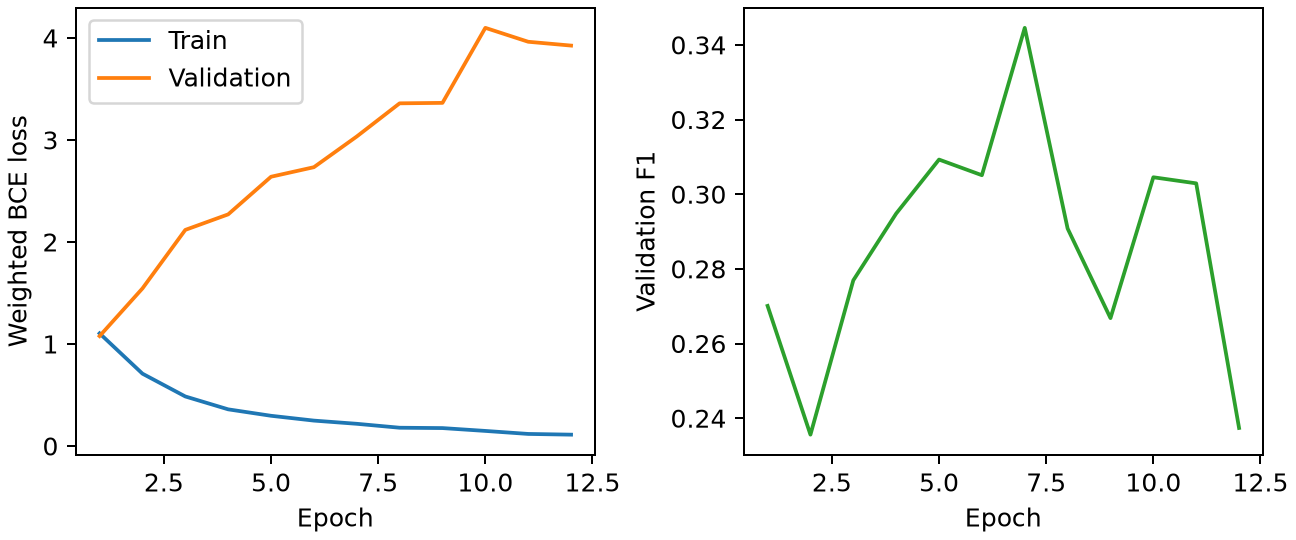
\includegraphics[width=0.86\linewidth]{figures/lstm_learning_curves.png}
  \caption{Selected LSTM training. Training loss falls while validation loss rises, showing rapid overfitting. The checkpoint is selected by validation F1, not final-epoch loss.}
  \label{fig:curves}
\end{figure}

\section*{Qualitative Results and Evaluation on New Data}

The 5,587 test windows come only from two recording dates that were excluded from preprocessing statistics, feature and window selection, checkpoints, thresholds, and hyperparameters. They are new temporal samples from the same two lobbies, not a third independently collected environment. This is a valid test of date shift but a narrower claim than cross-site deployment. Test confusion matrices are $[[4675,433],[343,136]]$ for logistic regression and $[[4771,337],[435,44]]$ for the LSTM, ordered as $[[TN,FP],[FN,TP]]$.

Four cases were selected deterministically by confusion-matrix category. A true positive approached from 0.87 to 0.58 m and slowed from 1.04 to 0.01 m/s; the LSTM assigned 0.988 probability. A false positive followed a similar approach-and-stop pattern but did not engage within four seconds ($p=0.991$). A false negative remained near 0.96 m with almost no motion before later engagement ($p<0.001$). A true negative also remained close and stationary ($p<0.001$). These examples show why proximity or stopping alone is insufficient and why some behavioral labels are ambiguous from a two-second observation.

\section*{Discussion}

The main result is a failure to generalize, not a neural-model improvement. The best-seed LSTM appeared to gain 0.060 validation F1 over logistic regression, but two additional seeds reduced the LSTM mean to 0.273. On unseen dates its recall fell to 9.2\%, while the simpler baseline retained 28.4\% recall. The rising validation loss in Figure~\ref{fig:curves}, high variance across seeds, and lobby/date subgroup differences point to overfitting and temporal distribution shift.

This task is difficult for three reasons. First, positives form only 5\% of windows. Second, the target is future engagement behavior, an imperfect proxy for internal intent. Similar approach-and-stop motion can receive opposite labels. Third, overlapping windows create many samples but fewer independent behaviors. Rich pose improved one LSTM seed but hurt logistic regression, so additional coordinates are not automatically informative. Future work should add independent locations and more positive tracks, evaluate at the track level, calibrate probabilities across dates, and test whether longer histories help once they do not reduce the dataset so sharply. For this deployment, the orientation logistic model is the more defensible choice.

\section*{Ethical Considerations}

Public-space observation creates privacy and consent concerns even when released data are de-identified. Kinect pose noise, behavioral imbalance, and two campus lobbies may also produce uneven errors for people or behaviors absent from training. A false positive can cause unwanted attention; a false negative can make the robot unresponsive. The system should therefore control only reversible actions such as a neutral greeting or waiting, retain no identifying imagery, expose an uncertainty-based option to abstain, and never support surveillance, access, employment, or safety-critical decisions.

\clearpage
\bibliographystyle{plainnat}
\bibliography{references}

\end{document}
